\chapter{外文资料的书面翻译}

\title{深度梯度压缩:为分布式训练减少通信带宽}

{\heiti 摘要:} 大规模分布式训练需要大量的通信带宽用于梯度交换,这限制了多节点训练的可扩展性,并且需要昂贵的高带宽网络基础设施。随着移动设备上的分布式训练(联合学习)的出现,情况变得更加糟糕,这种训练具有更高的延迟、更低的吞吐量和间歇性的不良连接。本文发现分布式SGD中99.9\%的梯度交换是冗余的,并提出深度梯度压缩(DGC)来大大降低通信带宽。为了在压缩过程中保持准确率,DGC采用了四种方法:动量修正、局部梯度修剪、动量因子掩蔽和预训练。我们已经将深度梯度压缩应用于图像分类、语音识别和语言模型,使用的数据集包括Cifar10、ImageNet、Penn Treebank和Librispeech Corpus。在这些场景下,深度梯度压缩实现了从270$\times$到600$\times$的梯度压缩比而不损失精度,将ResNet--50的梯度大小从97 MB削减到0.35 MB,对于DeepSpeech 从488 MB削减到0.74 MB,深度梯度压缩使得在廉价的1 Gbps以太网上进行大规模分布式训练成为可能,并方便了移动设备上的分布式训练。


\section{引言}
大规模分布式训练提高了更深和更大模型训练的生产效率。同步随机梯度下降(SGD)广泛用于分布式训练。通过增加训练节点的数量和利用数据并行性,可以显著减少对相同大小的训练数据的前向—反向传播的总计算时间。然而,梯度交换成本很高,这使计算时间的节省相形见绌,特别是对于计算与通信比例低的循环神经网络(RNN)。因此,网络带宽成为扩大分布式训练的一个重要瓶颈。当在移动设备上执行分布式训练时,这种带宽问题变得更加严重,例如联合学习。由于更好的隐私和更好的个性化,移动设备上的训练很有吸引力,但一个关键问题是,这些移动设备的网络带宽更低,网络时断时续,移动数据计划昂贵。

深度梯度压缩(DGC)通过压缩梯度来解决通信带宽问题,如图A-1所示。为了确保不损失精度,DGC在梯度稀疏化的基础上采用动量修正和局部梯度裁剪来保持模型性能。DGC还使用动量因子掩蔽和预训练来克服通信减少而造成的数据过时问题。

我们根据经验验证了深度梯度压缩在多种任务、模型和数据集上的应用:CNN用于图像分类(使用Cifar10和ImageNet),RNN用于语言模型(使用Librispeech Corpus)和语音识别(使用Librispeech Corpus)。这些实验表明,梯度可以压缩到600倍,而不损失精度,这比以前的工作高一个数量级。

\begin{figure}[t]
  \centering
  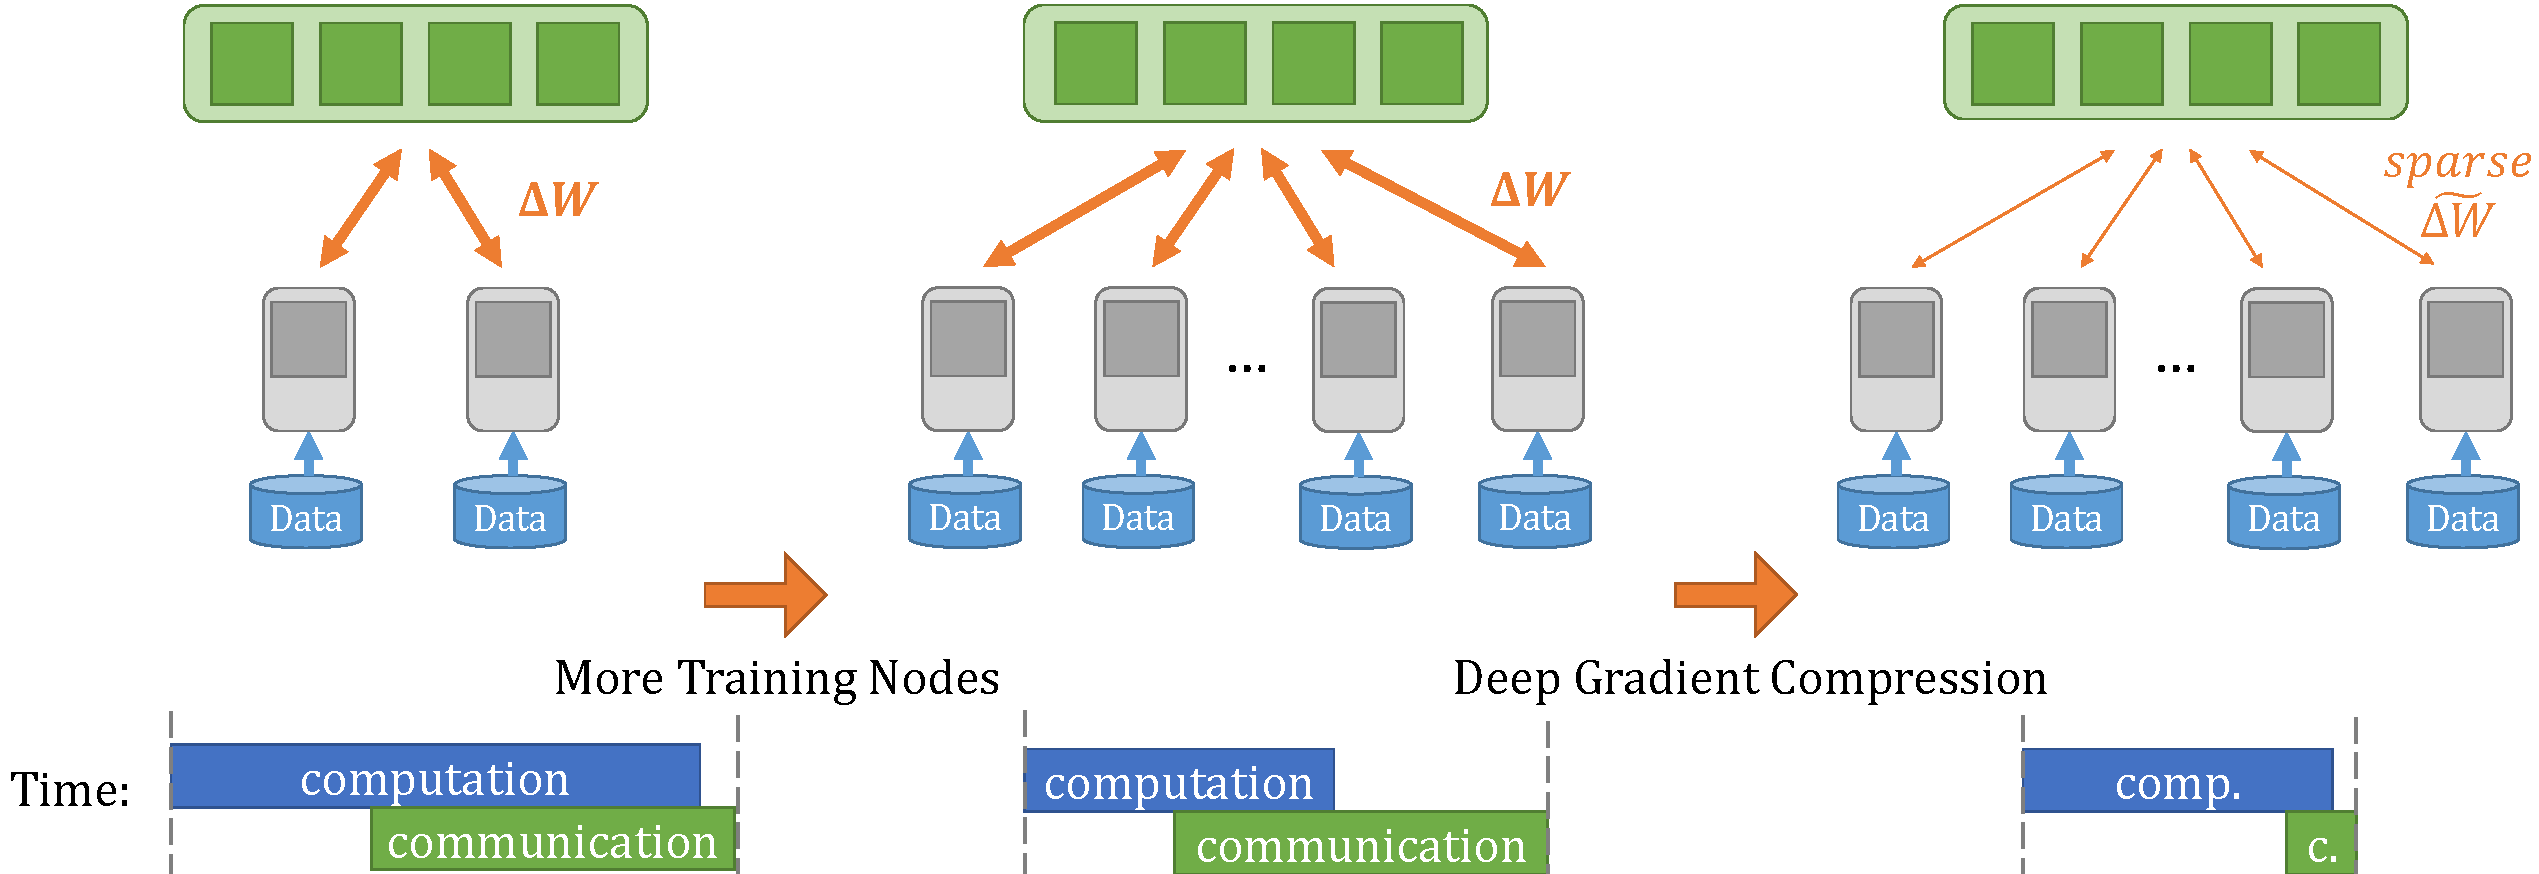
\includegraphics[width=\textwidth]{figures/dgc.pdf}
  \caption*{图~A-1\hskip1em 深度梯度压缩能够减少通信时间,提高可扩展性,并加速分布式训练}
  \label{fig:dgc}
\end{figure}

\section{相关工作}
研究人员提出了许多方法来克服分布式训练中的通信瓶颈。例如,一旦节点完成反向传播,异步SGD通过移除梯度同步和立即更新参数来加速训练。梯度量化和稀疏化以减少通信数据大小也被广泛研究。

\paragraph{梯度量化}
将梯度量化为低精度值可以降低通信带宽。Seide等人提出了1比特SGD来减小梯度传输数据大小,并在传统语音应用中实现了10倍的加速。Alistarh等人提出了另一种称为QSGD的方法,该方法对模型精度和梯度精度之间进行平衡。与QSGD相似,Wen等人开发了使用3级梯度的TernGrad。这两项工作都证明了量化训练的收敛性,尽管TernGrad只检测了CNN,而QSGD只检测了RNN的训练损失。也有人试图量化整个模型,包括梯度。DoReFa--Net使用1比特权重和2比特梯度。

\paragraph{梯度稀疏化}
Strom提出了阈值量化用来只发送大于预定常数阈值的梯度。然而,这个门槛在实践中很难选择。因此,Dryden等人分别选择了固定比例的正梯度和负梯度更新,Aji与Heafield提出梯度下降,以基于绝对值的单一阈值来稀疏梯度。为了保持收敛速度,梯度下降需要增加层归一化。梯度下降节省了99\%的梯度交换,同时导致机器翻译任务中BLEU分数损失0.3\%。同时,Chen等人提出根据局部梯度活动自动调整压缩率,对于全连通层,压缩率约为200倍,对于卷积层,压缩率约为40倍,而在ImageNet数据集上,top--1准确率的下降基本可以忽略不计。

与之前的工作相比,DGC将整个模型的梯度压缩比提高到600倍(所有层的压缩比相同)。DGC不需要额外的层正则化,因此不需要改变模型结构。最重要的是,深度梯度压缩不会导致精度损失。

\section{深度梯度压缩}

\subsection{梯度稀疏化}


\begin{figure}[!t]
  \vspace{-10pt}
  \begin{minipage}[H]{.5\textwidth}
    \begin{algorithm}[H] \footnotesize 
      \caption*{{\textbf{Algorithm~A-1}\hskip1em \small 节点$k$上的梯度稀疏化}}
      \label{alg:ssgd}
      \begin{algorithmic}[1]
        \Require dataset $\chi$
        \Require minibatch size $b$ per node
        \Require the number of nodes $N$
        \Require optimization function $SGD$
        \Require init parameters $w = \{w[0], w[1], \cdots, w[M]\}$
        \State $G^{k} \gets 0$
        \For{$t=0,1,\cdots$}
        \State $G_{t}^{k} \gets G_{t-1}^{k}$
        \For{$i=1,\cdots,b$}
        \State Sample data $x$ from $\chi$
        \State $G_{t}^{k} \gets G_{t}^{k} + \frac{1}{Nb} \triangledown f \left(x;w_{t} \right) $
        \EndFor
        \For{$j=0, \cdots, M$}
        \State Select threshold: $thr \gets s\%$ of $\left|G_{t}^{k}[j]\right|$
        \State $ Mask \gets \left|G_{t}^{k}[j]\right| > thr$
        \State $\widetilde{G}_{t}^{k}[j] \gets G_{t}^{k}[j] \odot Mask$
        \State $G_{t}^{k}[j] \gets G_{t}^{k}[j] \odot \neg Mask$
        \EndFor
        \State  \emph{All-reduce} $G_{t}^{k}$ : $G_{t} \gets \sum_{k=1}^{N} encode(\widetilde{G}_{t}^{k})$
        \State $w_{t+1} \gets \emph{SGD} \left(w_{t}, G_{t} \right)$
        \EndFor
      \end{algorithmic}
    \end{algorithm}
  \end{minipage}
  \hspace{15pt}
  \begin{minipage}[H]{.4\linewidth}
    \begin{figure}[H]
      \begin{subfigure}{6cm}
      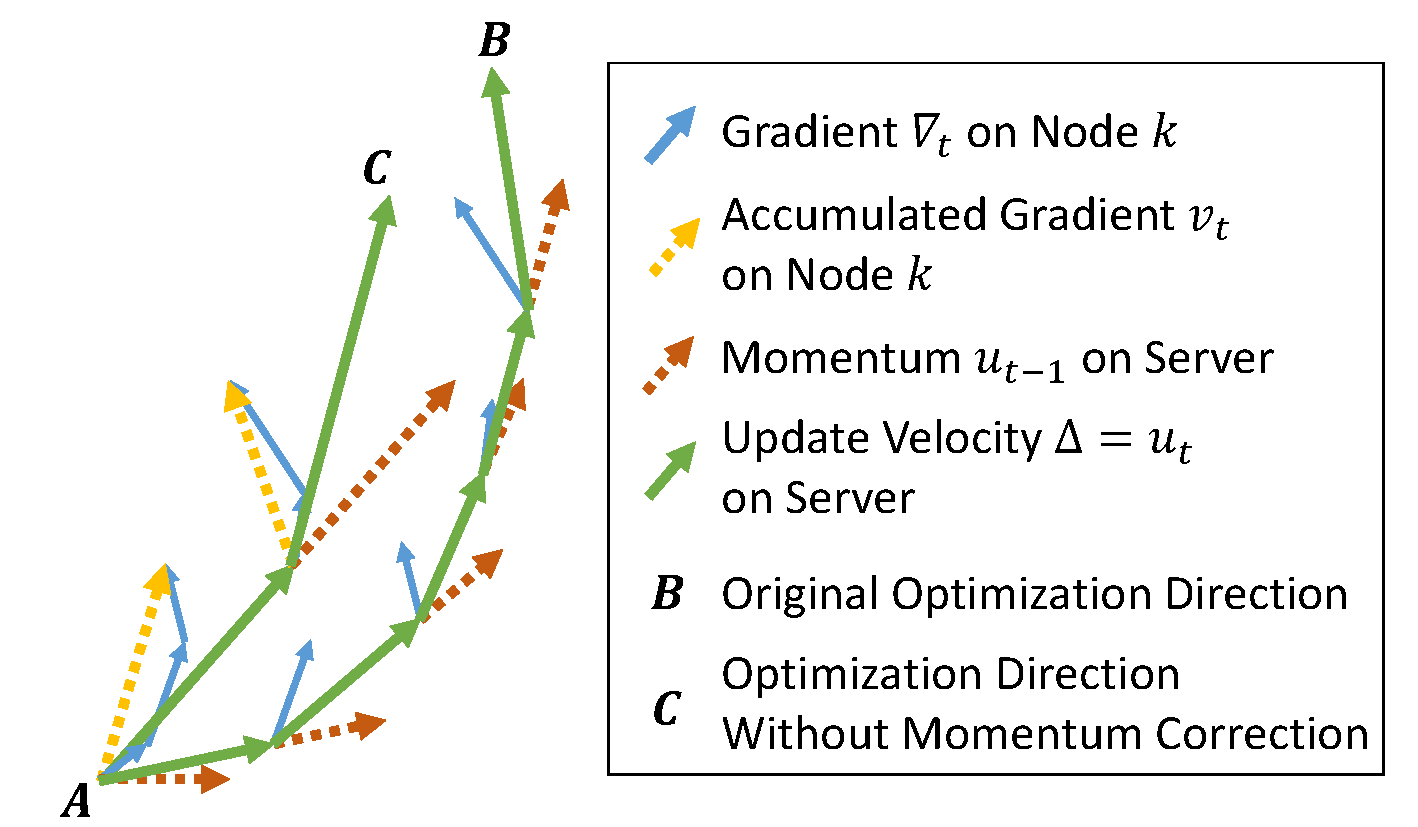
\includegraphics[width=\linewidth]{figures/msgd_1.pdf}\label{fig:msgd_nomc}
      \caption{不使用动量矫正的局部梯度累积}
      \end{subfigure}
      \begin{subfigure}{6cm}
      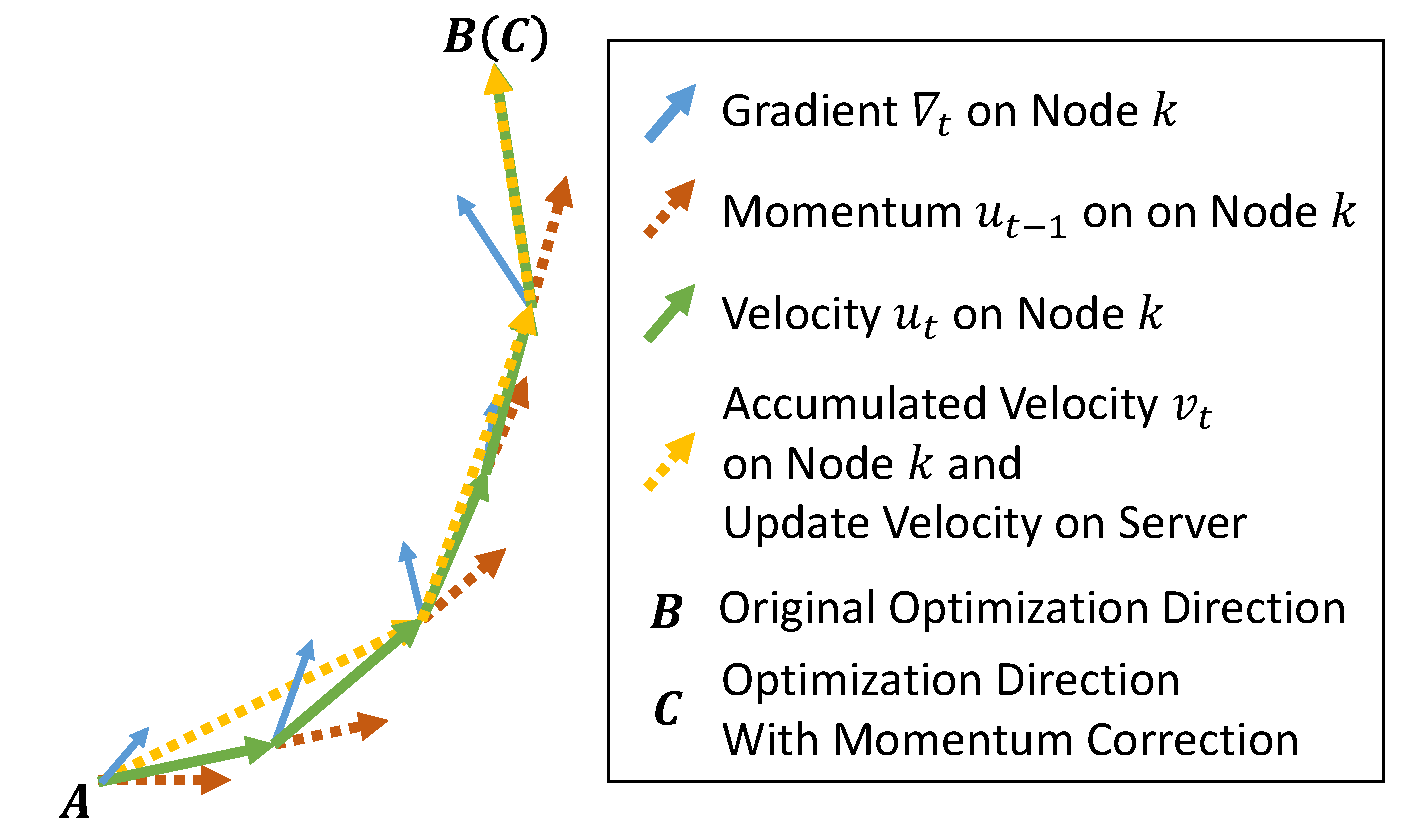
\includegraphics[width=\linewidth]{figures/msgd_2.pdf}\label{fig:msgd_mc}
      \caption{使用动量矫正的局部梯度累积}
      \end{subfigure}
      \caption*{图~A-2\hskip1em 动量矫正}
    \end{figure}
  \end{minipage}
\end{figure}


我们通过只发送重要的梯度(稀疏更新)来减少通信带宽。我们使用基于梯度绝对值的简单启发式算法:仅传输大于阈值的梯度。为了避免丢失信息,我们在本地积累其余的梯度。最终,这些梯度变得足够大,可以传输。因此,我们立即发送大梯度,但最终会发送所有梯度,如算法1所示。$encode()$函数包含32位非零梯度值和16位游程长度。我们的关电视,局部梯度累积相当于随着时间的推移增加批大小(batch size)。令$F(w)$为我们想要优化的损失函数。同步分布式SGD通过总共N个训练节点执行以下更新:

\begin{equation}
	\label{eq:dsgd}
	F(w) = \frac{1}{\left|\chi \right|} \sum_{x \in \chi} f(x, w), \qquad
	w_{t+1} = w_{t} - \eta \frac{1}{Nb} \sum_{k=1}^{N}\sum_{x \in \mathcal{B}_{k, t}} \triangledown f(x, w_{t})
\end{equation}

其中$\chi$是训练数据集,$w$是网络的权重,$f(x,w)$是根据样本$x$计算的损失,$x$从$\chi$中采样,$\eta$是学习率,$N$是训练节点的数量,对于$1 \leq k \le N$的$B_k$ 是一个在第$t$轮迭代时从$\chi$中采样的长为$N$的迷你批次(mini batch)序列,每个大小为$b$。

考虑展开后的权重$w$中第$i$个位置的权重$w^{(i)}$。经过$T$轮迭代后,我们有:
\begin{equation}
	\label{eq:titer}
	w_{t+T}^{(i)} = w_{t}^{(i)} - \eta T \cdot \frac{1}{NbT} \sum_{k=1}^{N} \left (\sum_{\tau=0}^{T-1}\sum_{x \in \mathcal{B}_{k, t+\tau}} \triangledown^{(i)} f(x, w_{t+\tau}) \right ) 
\end{equation}

等式A-2表明,局部梯度累积可以被认为是将批大小从$Nb$增加到$NbT$($\tau$上的第二次求和),其中$T$是发送$w^{(i)}$梯度的两次迭代之间的\emph{稀疏更新间隔}的长度。学习率缩放是处理大型迷你批次的常用技术。学习速率$\eta T$和批大小$NbT$中的$T$被抵消,在等式A-2中自动满足。

\subsection{提高局部梯度累计}
如果不注意的话,当稀疏度非常高时,稀疏更新将极大地影响收敛。例如,算法1对Cifar10数据集造成了超过1.0\%的准确率损失,如图A-5(a)所示。我们发现动量修正和局部梯度修剪可以缓解这个问题。

\paragraph{动量修正}
动量SGD被广泛用于代替朴素SGD。然而,算法1并不直接应用于带有动量项的SGD,因为它忽略了稀疏更新间隔之间的折扣因子。

随后是在N个训练节点上使用朴素SGD的分布式训练,

\begin{equation}
	\label{eq:msgd}
	u_{t} = mu_{t-1} + \sum_{k=1}^{N}\left( \triangledown_{k,t}\right),\quad  w_{t+1} = w_{t} - \eta u_{t}
\end{equation}

其中$m$是动量,$N$是训练节点的数量,并且$\triangledown_{k,t} =  \frac{1}{Nb} \sum_{x \in \mathcal{B}_{k, t}} \triangledown f(x, w_{t})$。

考虑展开后的权重$w$中的第$i$个位置的权重$w^{(i)}$。在经过$T$轮迭代之后,权重$w^{(i)}$的变化如下所示:

\begin{equation}
	\label{eq:msgd_change}
	w_{t+T}^{(i)} = w_{t}^{(i)} - \eta \left[\cdots +  \left( \sum_{\tau=0}^{T-2} m^{\tau}\right)\triangledown^{(i)}_{k,t+1} + \left( \sum_{\tau=0}^{T-1} m^{\tau}\right)\triangledown^{(i)}_{k,t}\right]
\end{equation}

如果具有动量的SGD直接应用于稀疏梯度场景(算法1中的第15行),更新规则不再等同于等式A-3,等式A-3变为:

\begin{equation}
	\label{eq:nomc}
	v_{k,t} = v_{k,t-1} + \triangledown_{k, t},\quad u_{t} = mu_{t-1} + \sum_{k=1}^{N} sparse\left( v_{k, t}\right) ,\quad  w_{t+1} = w_{t} - \eta u_{t}
\end{equation}

其中第一项是训练节点$k$上的局部梯度累积。一旦累计结果$v_{k,t}$大于阈值,它将向$sparse()$函数传递硬阈值(hard thresholding),并在第二项中被编码并通过网络发送。类似于算法1中的第12行,累加结果$v_{k,t}$被$sparse()$函数中的掩码清除。

稀疏更新间隔$T$之后权重值$w^{(i)}$的变化变成,

\begin{equation}
	\label{eq:nomc_change}
	w_{t+T}^{(i)} = w_{t}^{(i)} - \eta \left(\cdots + \triangledown^{(i)}_{k,t+1} + \triangledown^{(i)}_{k,t}\right)
\end{equation}

与等式A-4相比,等式A-6中累积折扣因子$\sum_{\tau=0}^{T-1} m^{\tau}$的消失导致收敛性能的损失。如图A-2(a)所示,等式A-4实现了从点$A$到点$B$的优化,但是有了局部梯度累积,等式A-4转到点$C$。当梯度稀疏度较高时,更新间隔$T$显著增加,因此显著的副作用将损害模型性能。为了避免这个错误,我们需要在公式5的基础上进行动量修正,以确保稀疏更新等同于公式3中的密集更新。

如果我们把方程3中的速度$u_t$看作“梯度”,方程3的第二项可以被认为是“梯度”$u_t$的朴素SGD。在第3.1节中,局部梯度累积被证明对朴素的SGD是有效的。因此,我们可以在局部累加速度$u_t$,而不是实际的梯度$\triangledown_{k,t}$,来将等式A-5迁移到等式A-3:

\begin{equation}
	\label{eq:mc}
	u_{k,t} = mu_{k,t-1} + \triangledown_{k,t},\quad  v_{k,t} = v_{k,t-1} + u_{k,t},\quad   w_{t+1} = w_{t} - \eta \sum_{k=1}^{N} sparse\left( v_{k,t}\right) 
\end{equation}

其中前两项是校正的局部梯度累积和累积结果$v_{k,t}$,它们倍用于随后的稀疏化和通信。通过局部累积的这一简单变化,我们可以从等式A-7推导出等式A-4中累积折扣因子$\sum_{\tau=0}^{T-1} m^{\tau}$,如图A-2(b)所示。

我们称这种迁移为\emph{动量修正}。这是对更新公式的一个调整,不会产生任何超参数。除了朴素的动量SGD之外,我们还在附录B中考察了内斯特罗夫动量SGD,它类似于动量SGD。

\paragraph{局部梯度裁剪}
梯度裁剪被广泛采用以避免爆炸梯度问题。 Pascanu等人提出的方法只要其L2范数的总和超过阈值,就重新调整梯度。 通常在来自所有节点的梯度聚合之后执行该步骤。 因为我们独立地在每个节点上的迭代上累积梯度,所以我们在将当前梯度$G_t$添加到先前累积(算法1中的$G_{t-1}$)之前在本地执行梯度裁剪。 如附录C中所述,如果所有$N$个节点具有相同的梯度分布,我们就将阈值缩放$N^{-1/2}$,即当前节点的全局阈值的分数。 在实践中,我们发现局部梯度裁剪的行为与训练中的朴素梯度裁剪非常相似,这表明我们的假设在实际数据中可能是有效的。

正如我们将在第4节中看到的那样,动量校正和局部梯度裁剪有助于将AN4语料库的单词错误率从14.1%降低到12.9%,而训练曲线更接近动量SGD。

\subsection{克服数据过时的影响}
因为我们延迟了小梯度的更新,当这些更新发生时,它们就过时了。在我们的实验中,当梯度稀疏度为99.9\%时,大多数参数每600到1000次迭代更新一次,这与每个epoch的迭代次数相比而言相当长。数据过时效应会减慢收敛速度并降低模型性能。我们通过动量因子掩蔽和预训练来缓解较少数据过时效应。

\paragraph{动量因子掩蔽}
Mitliagkas等人讨论了异步导致的过时问题,并将其归因于一个被描述为\emph{隐式动量}的术语。受他们工作的启发,我们引入动量因子掩蔽,以缓解数据过时性。我们没有像Mitliagkas等人所建议的那样搜索新的动量系数,而是简单地对累积梯度$v_{k,t}$和等式A-7中的动量因子$u_{k,t}$应用相同的掩码:

\begin{equation*}
  Mask \gets |v_{k,t}| >thr,\quad v_{k,t} \gets v_{k,t} \odot \neg Mask, \quad u_{k,t} \gets u_{k,t} \odot \neg Mask
\end{equation*}

这个掩码阻止了延迟梯度的动量,防止了过时的动量将权重带向错误的方向。

\paragraph{预训练}
在训练的早期阶段,网络变化迅速,梯度更加多样和积极。稀疏梯度限制了模型的变化范围,从而延长了网络剧烈变化的周期。同时,在被选择用于下一次更新之前,来自早期阶段的剩余的绝对值较大的梯度被累积,因此它们可能超过最新梯度并误导优化方向。大规模的迷你批次训练中引入的\emph{预训练}方法对此很有帮助。在预训练阶段,我们使用比较不积极的学习速率来降低训练开始时神经网络的变化速度,并且使用比较不积极的梯度稀疏性来减少被延迟的极端梯度的数量。为了帮助训练适应较大稀疏度的梯度,我们不是在前几个时期线性增加学习率,而是指数地将梯度稀疏度从相对较小的值增加到最终值。

\begin{figure}[ht]
  \centering
  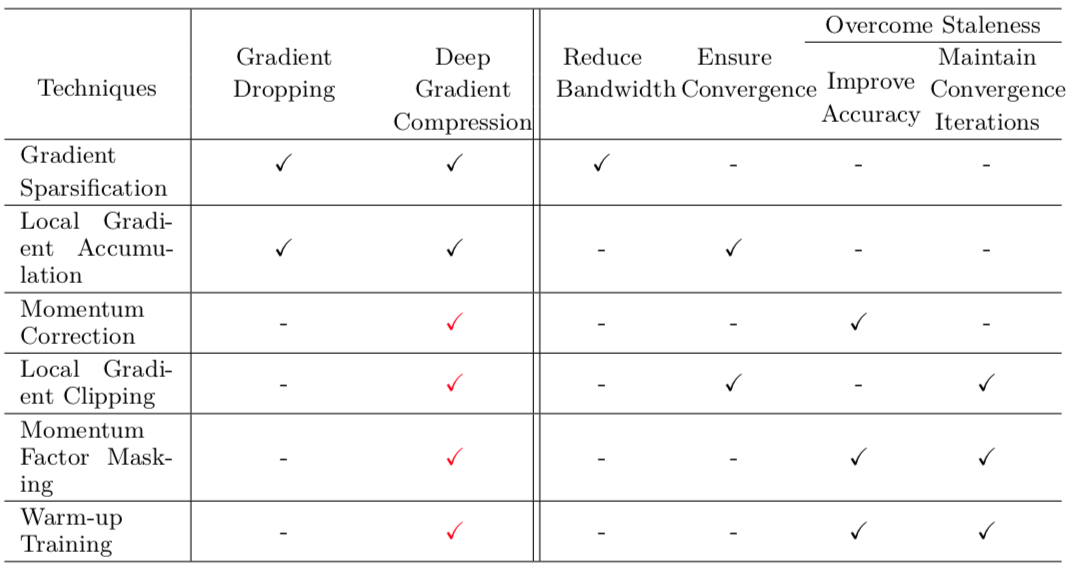
\includegraphics[width=\textwidth]{figures/table1.png}
  \caption*{图~A-3\hskip1em 深度梯度压缩中使用的技术}
  \label{fig:table1}
\end{figure}

如图A-3所示,动量修正和局部梯度修剪改善了局部梯度积累,而动量因子掩蔽和热身训练减轻了数据过时效应。除了梯度稀疏化和局部梯度累积之外,这四种技术组成了深度梯度压缩(附录D中的伪代码),并有助于在保持精度的同时提高梯度压缩比。

\section{实验}
\subsection{实验设置}
我们在三种机器学习任务上验证了我们的方法:Cifar10和ImageNet上的图像分类,Penn Treebank数据集上的语言模型,AN4和Librispeech语料库上的语音识别。深度梯度压缩引入的唯一超参数是预训练策略。在所有与DGC相关的实验中,预热阶段的稀疏度分别为:75\%、93.75\%、98.4375\%、99.6\%、99.9\%(指数增长至99.9\%)。我们通过梯度压缩比例评估网络带宽的降低情况如下:

\begin{equation*}
  \text{Gradient Compression Ratio} = size\left[encode\left(sparse({G}^k)\right)\right] / size\left[ G^k \right]
\end{equation*}

其中$G^k$是在训练节点k上计算的梯度。

\paragraph{图像分类}
我们研究了Cifar10上的ResNet--110,ImageNet上的AlexNet和ResNet--50。Cifar10由10个类中的50,000个训练图像和10,000个验证图像组成,而ImageNet包含1000个类中的100多万个训练图像和50,000个验证图像。我们按照Gross 和 Wilber提出的训练方法,使用动量SGD进行模型训练。DGC的预训练阶段是Cifar10的164个epoch中的4个epoch,以及ImageNet数据集的90个epoch中的4个epoch。

\paragraph{语言模型}
Peen Treebank语料库(PTB)数据集由923,000个训练、73,000个验证和82,000个测试词组成。我们选择的词汇与Mikolov等人选择的词汇相同。我们采用每层1500个隐藏单元的2层LSTM语言模型架构,按照Inan等人的建议,结合编码器和解码器的权重,并使用带有梯度修剪的\emph{朴素SGD},而当验证损失没有改善时,将学习率下降。预训练阶段是40个epoch中的1个epoch。

\paragraph{语音识别}
AN4数据集包含948个训练和130个测试话语,而Librispeech语料库包含960小时的阅读语音。我们使用没有n-gram语言模型的DeepSpeech结构,这是一个遵循卷积层堆积的多层RNN。我们为AN4训练一个每层800个隐藏单位的5层LSTM,为LibriSpeech训练一个每层1200个隐藏单位的7层GRU,采用内斯特罗夫动量梯度和梯度修剪,同时学习率在每个epoch都进行减少。DGC的预训练阶段是80个epoch中的1个epoch。

\subsection{结果与分析}

\begin{figure}[ht]
  \centering
  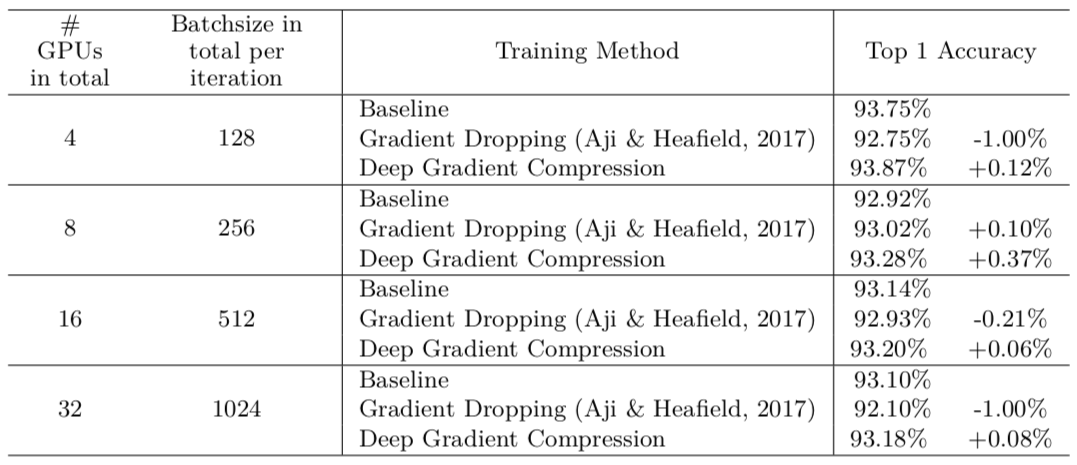
\includegraphics[width=\textwidth]{figures/table2.png}
  \caption*{图~A-4\hskip1em ResNet-101训练Cifar10数据集}
  \label{fig:table2}
\end{figure}

\begin{figure}[ht]
  \centering
  \label{fig:image_class}
  \begin{subfigure}{7cm}
    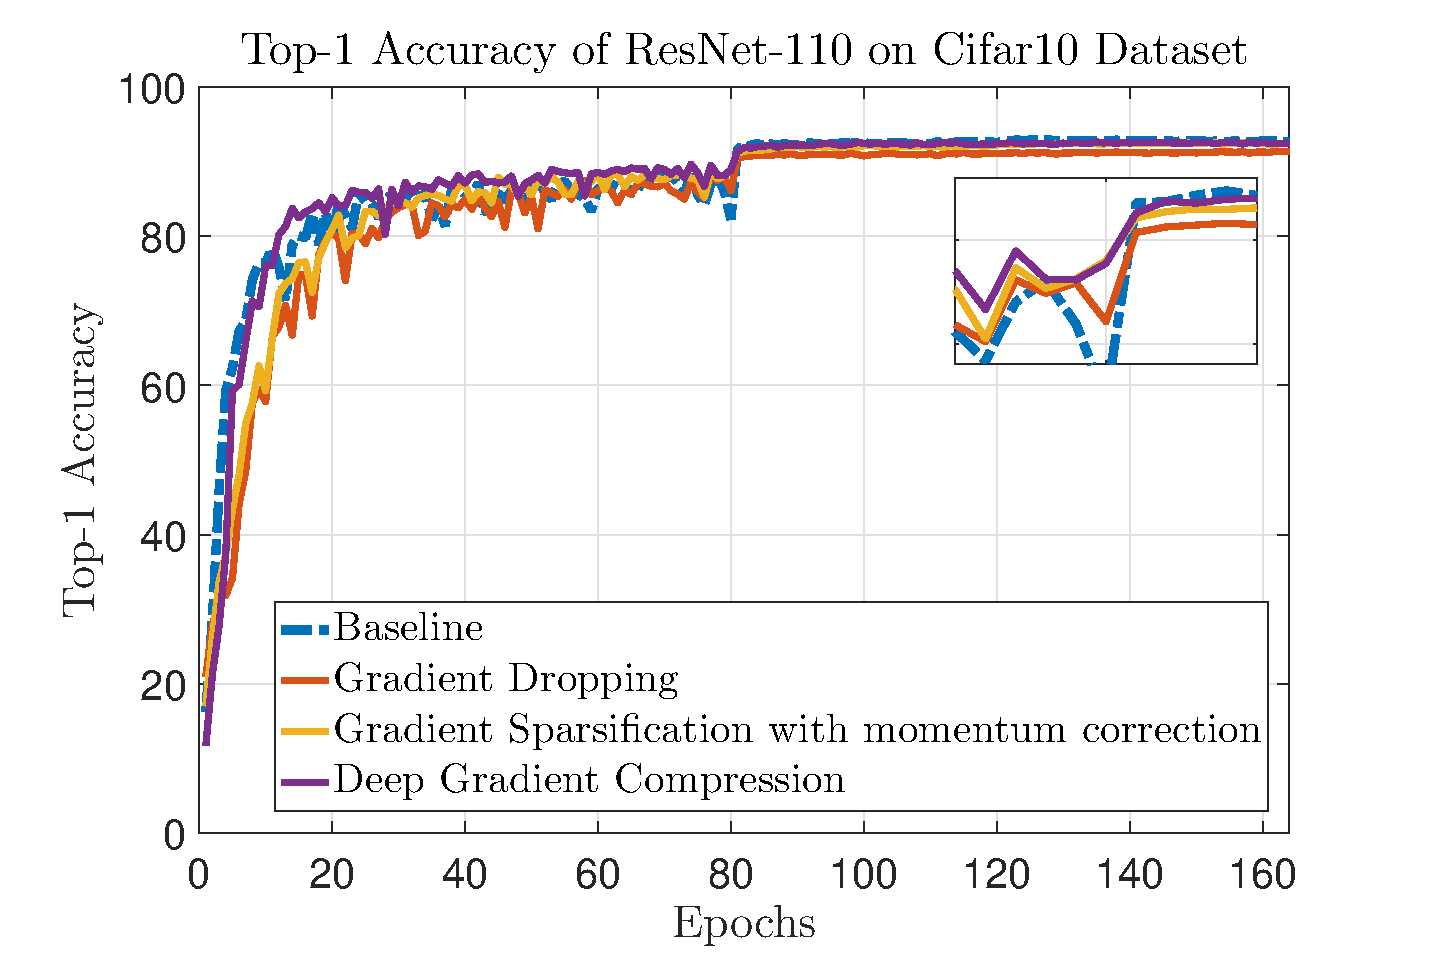
\includegraphics[width=\textwidth]{figures/cf_top1.eps}\label{fig:cf1}\caption{ResNet-101在Cifar10上的Top-1 准确率}
  \end{subfigure}
  \begin{subfigure}{7cm}
    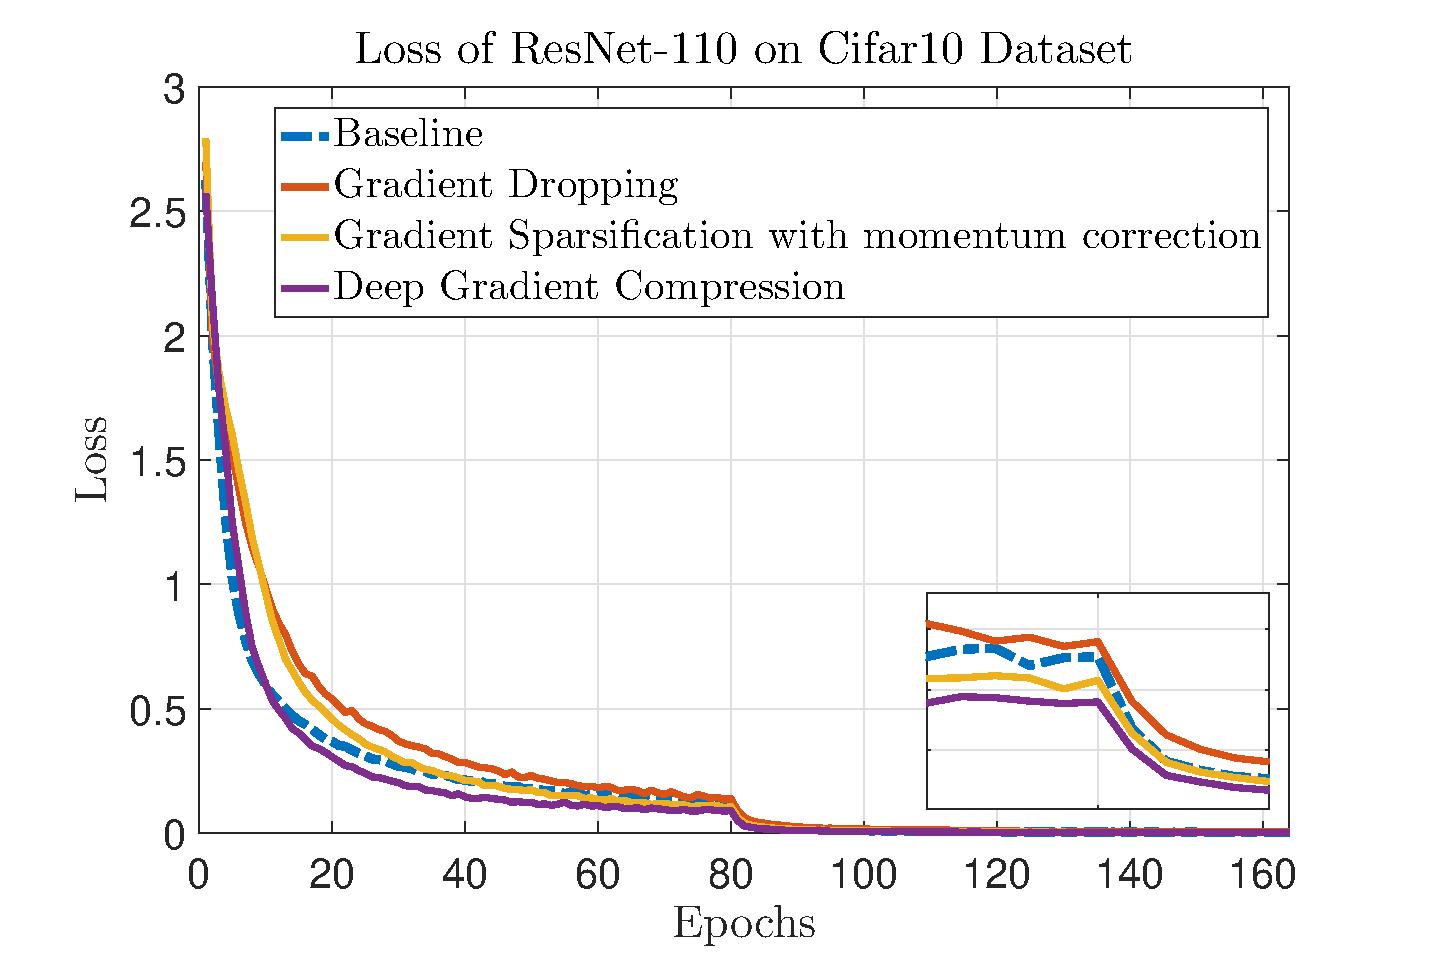
\includegraphics[width=\textwidth]{figures/cf_loss.eps}\label{fig:cf2}\\[-2ex]
    \caption{ResNet-101在Cifar10上的训练损失}
  \end{subfigure}
  \begin{subfigure}{7cm}
    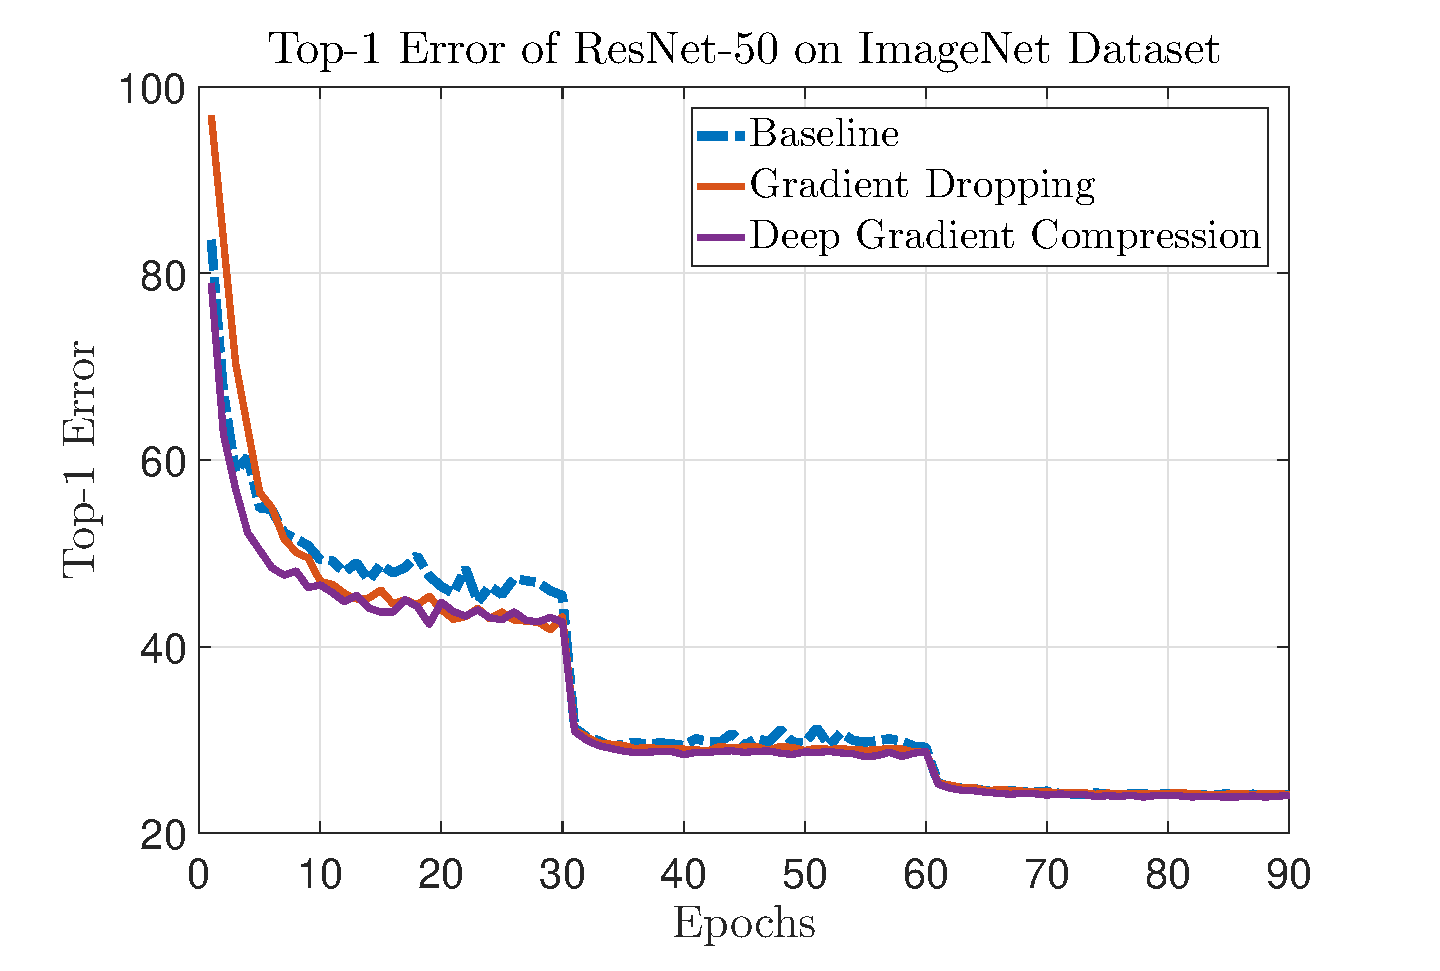
\includegraphics[width=\textwidth]{figures/im_top1.eps}\label{fig:im1}\caption{ResNet-50在Cifar10上的Top-1 错误率}
  \end{subfigure}
  \begin{subfigure}{7cm}
    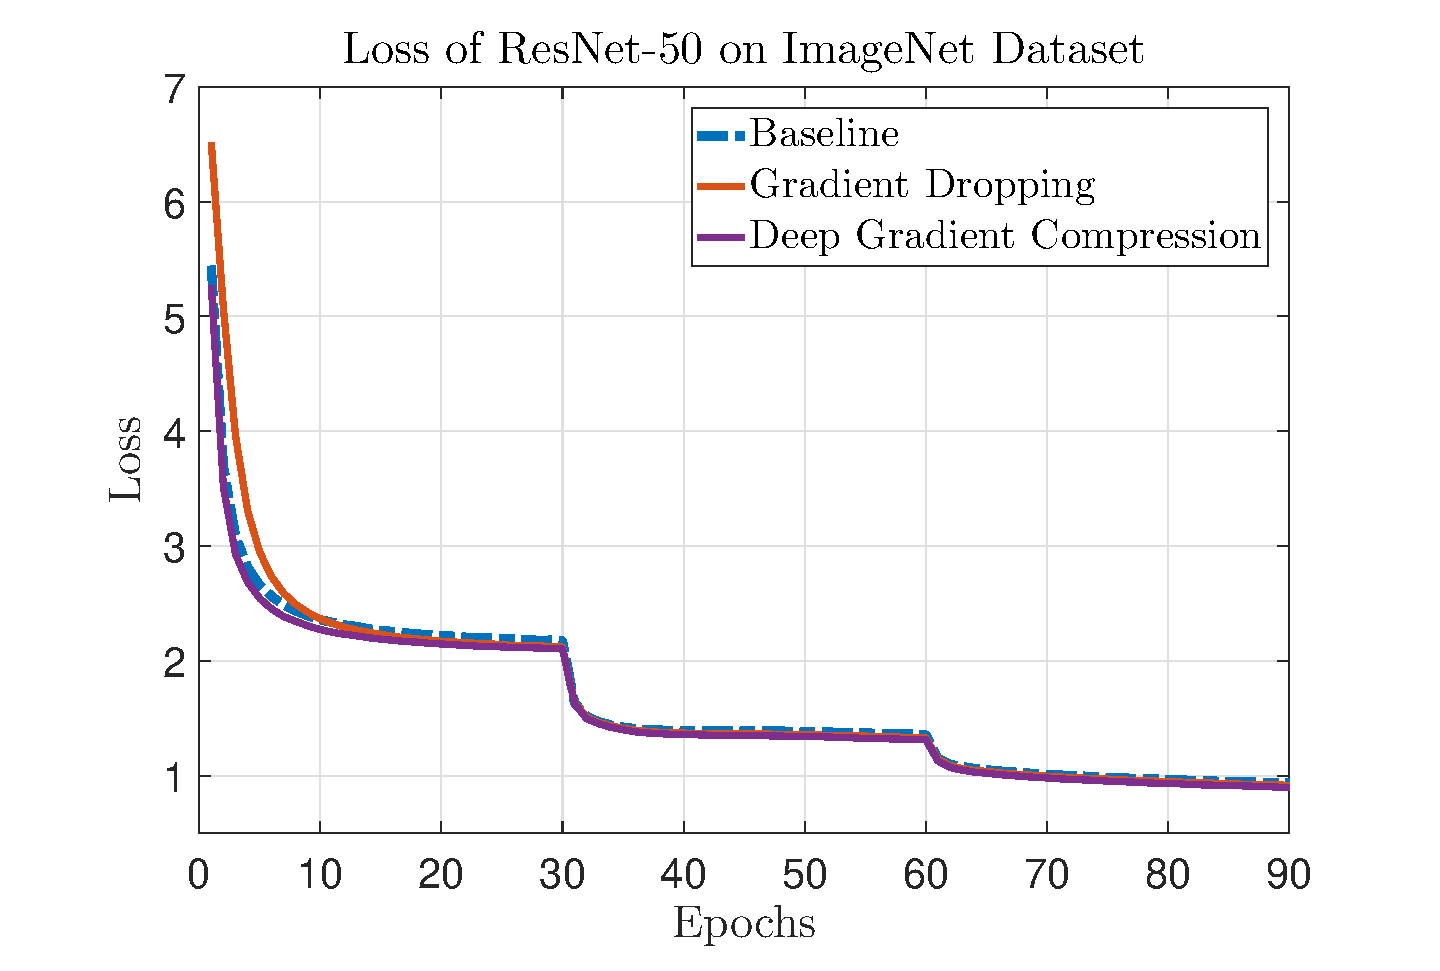
\includegraphics[width=\textwidth]{figures/im_loss.eps}\label{fig:im2}\caption{ResNet-50在Cifar10上的训练损失}
  \end{subfigure}
  \caption*{图~A-5 ResNet在图像分类任务中的学习曲线(梯度的稀疏度为99.9\%)}
\end{figure}

\begin{figure}[ht]
  \centering
  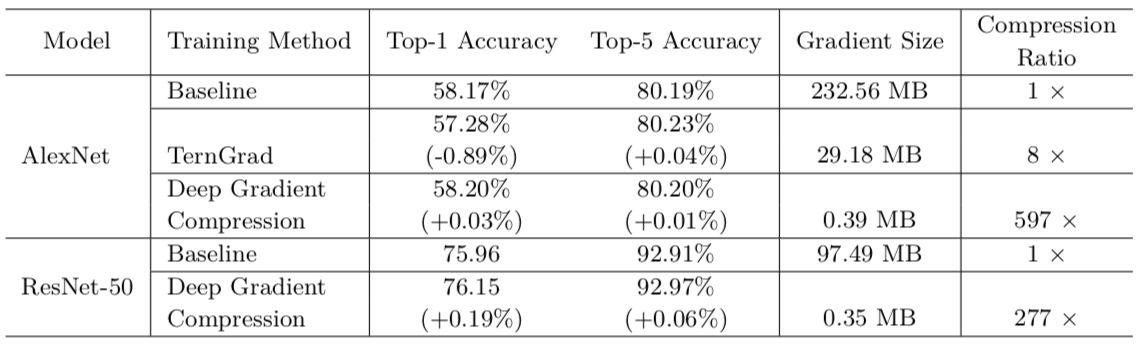
\includegraphics[width=\textwidth]{figures/table3.png}
  \caption*{图~A-6\hskip1em 在ImageNet数据集上对比梯度压缩率}
  \label{fig:table3}
\end{figure}

\begin{figure}[ht]
  \centering
  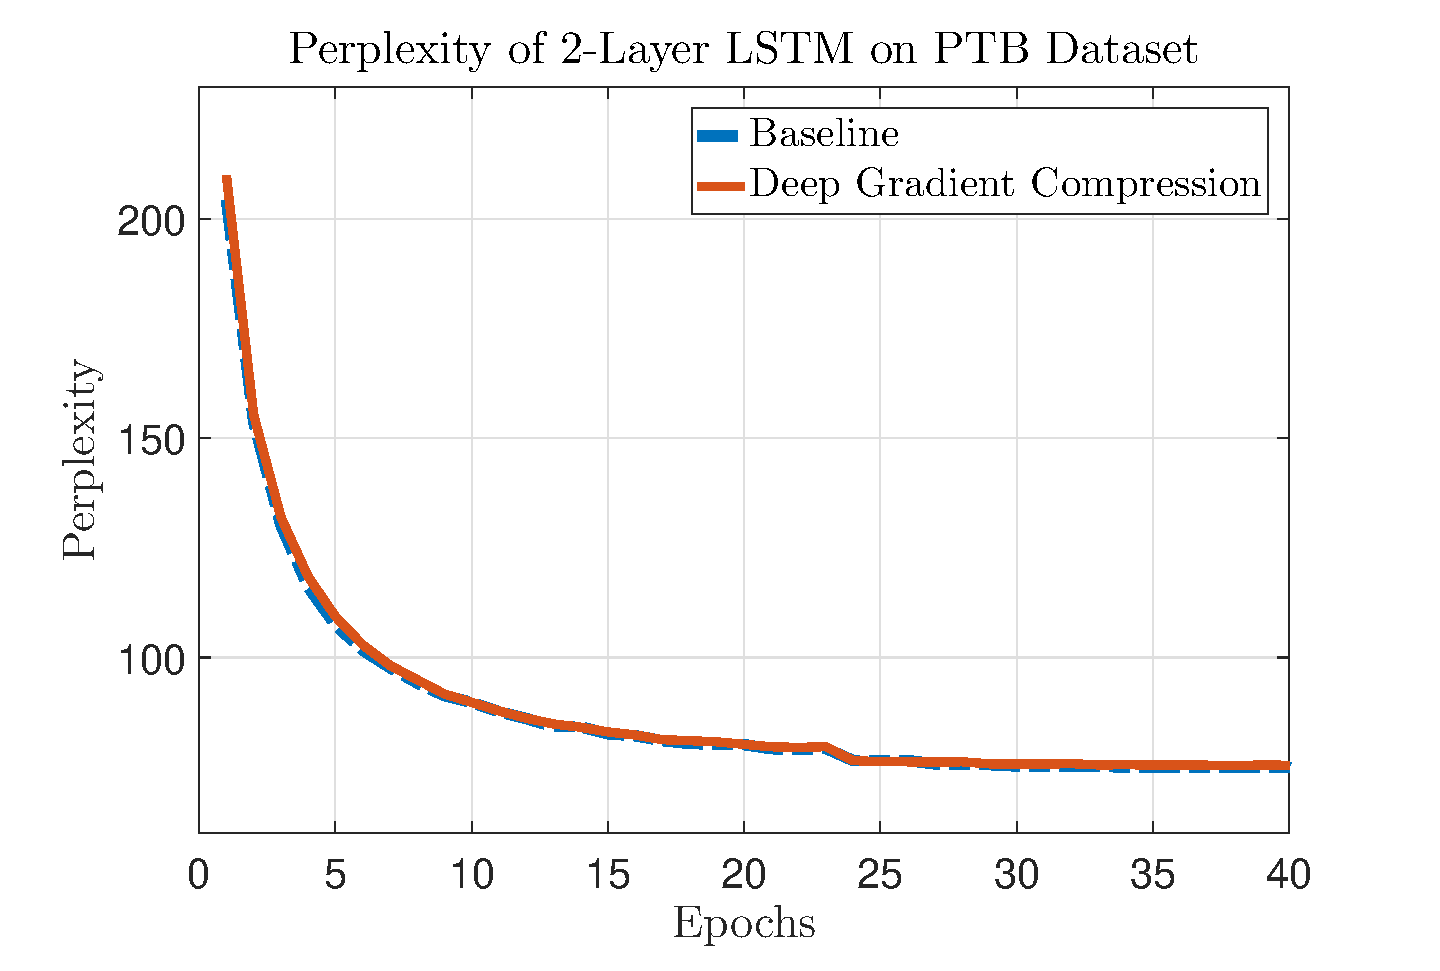
\includegraphics[width=0.49\textwidth]{figures/lm_ppl.eps}
  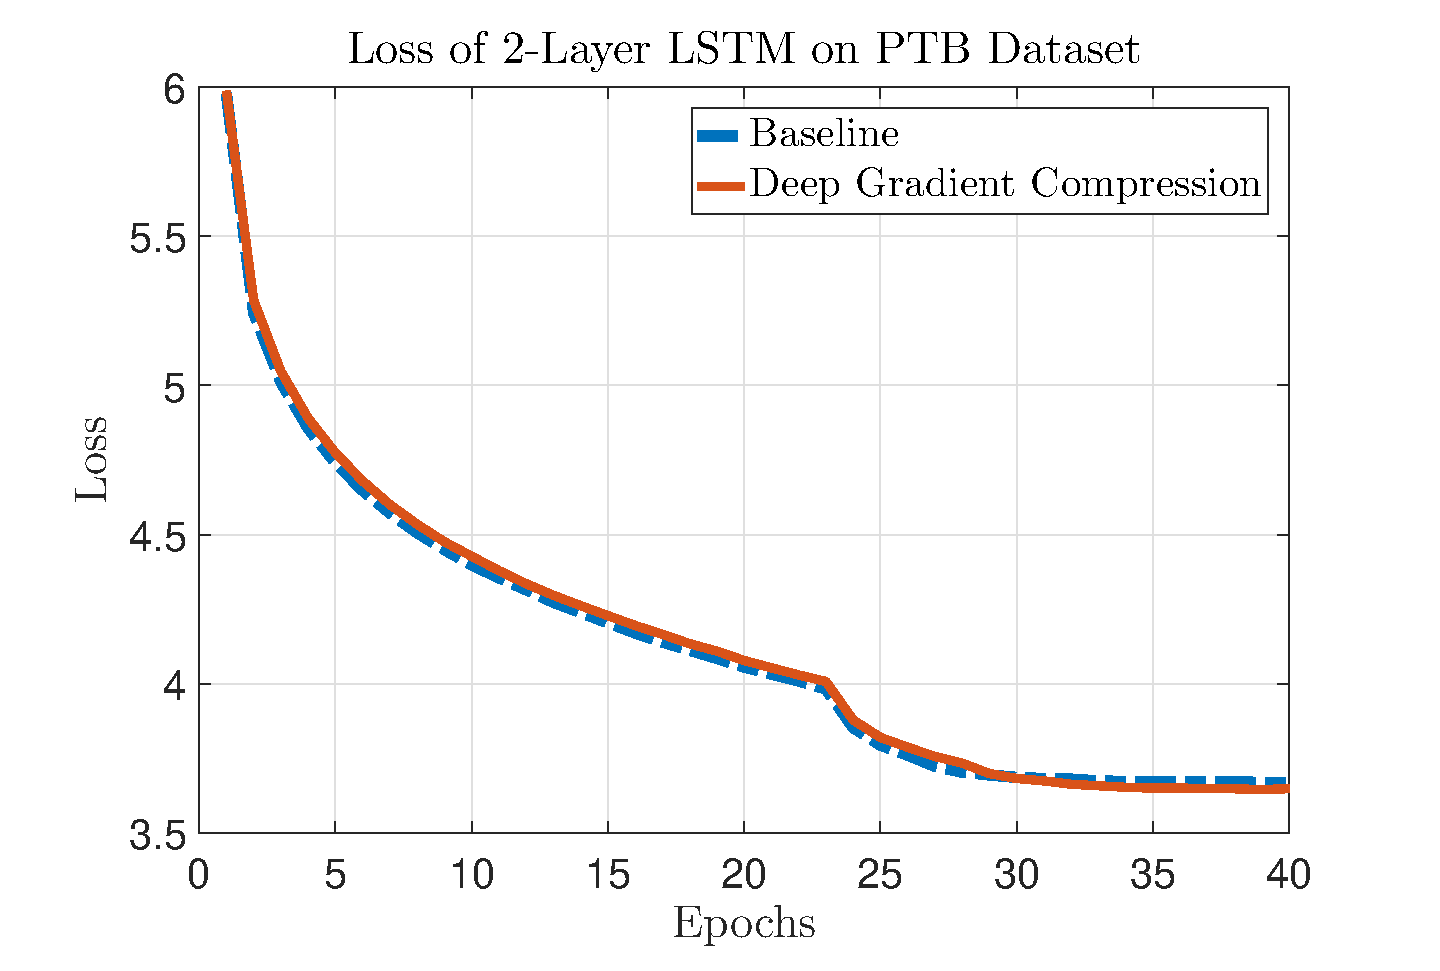
\includegraphics[width=0.49\textwidth]{figures/lm_loss.eps}
  \caption*{图~A-7\hskip1em LSTM语言模型在PTB数据集上的困惑度和训练损失(梯度稀疏度为99.9\%)}
  \label{fig:lm}
\end{figure}
\begin{figure}[ht]
  \centering
  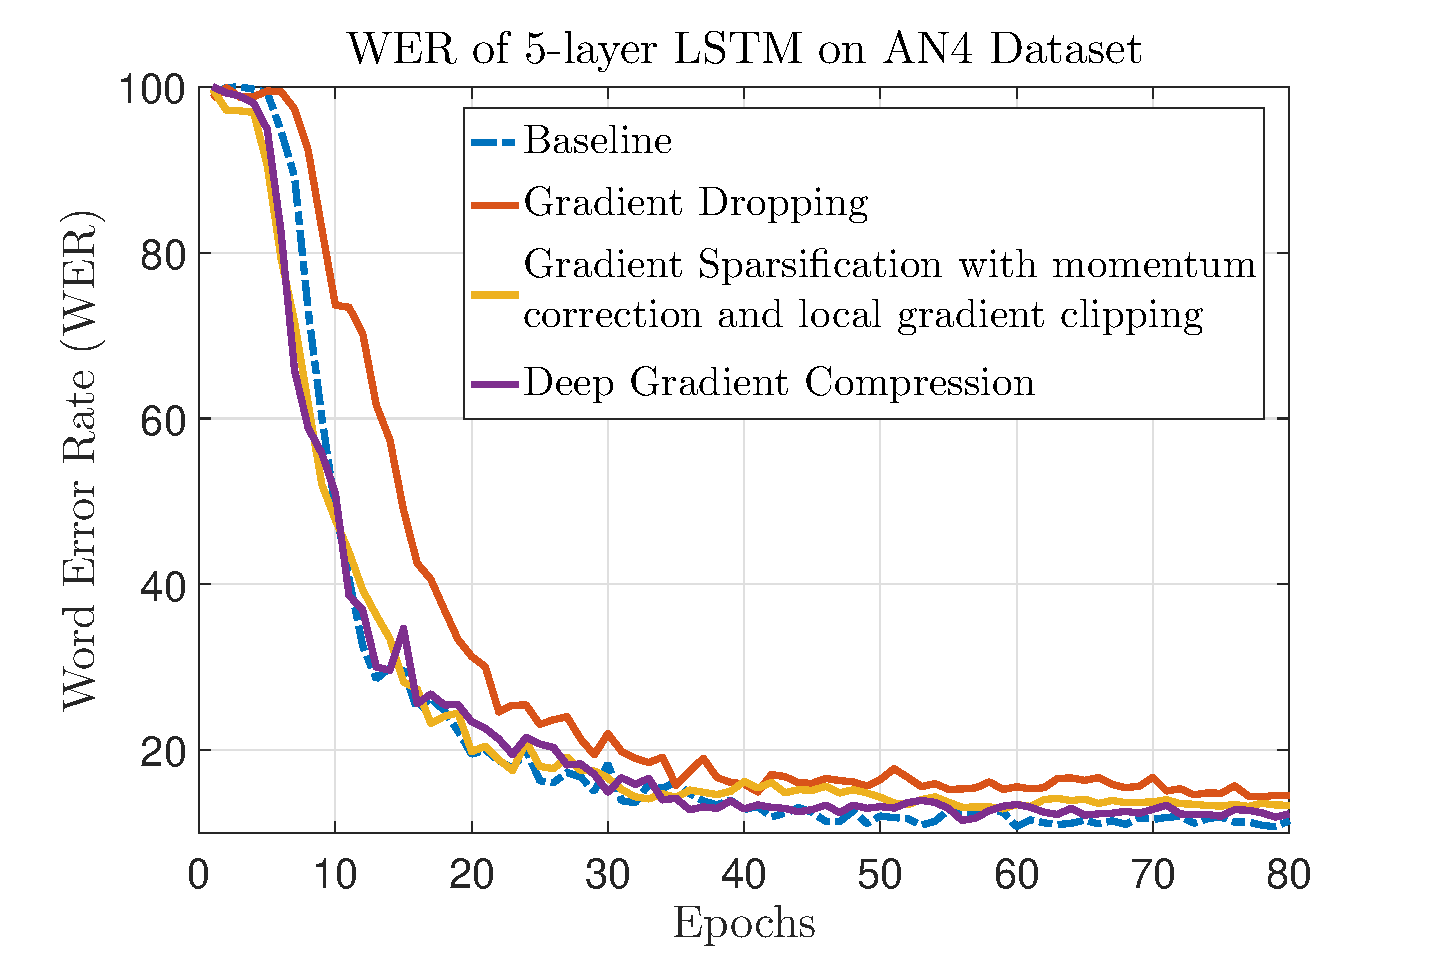
\includegraphics[width=0.49\textwidth]{figures/an_wer.eps}
  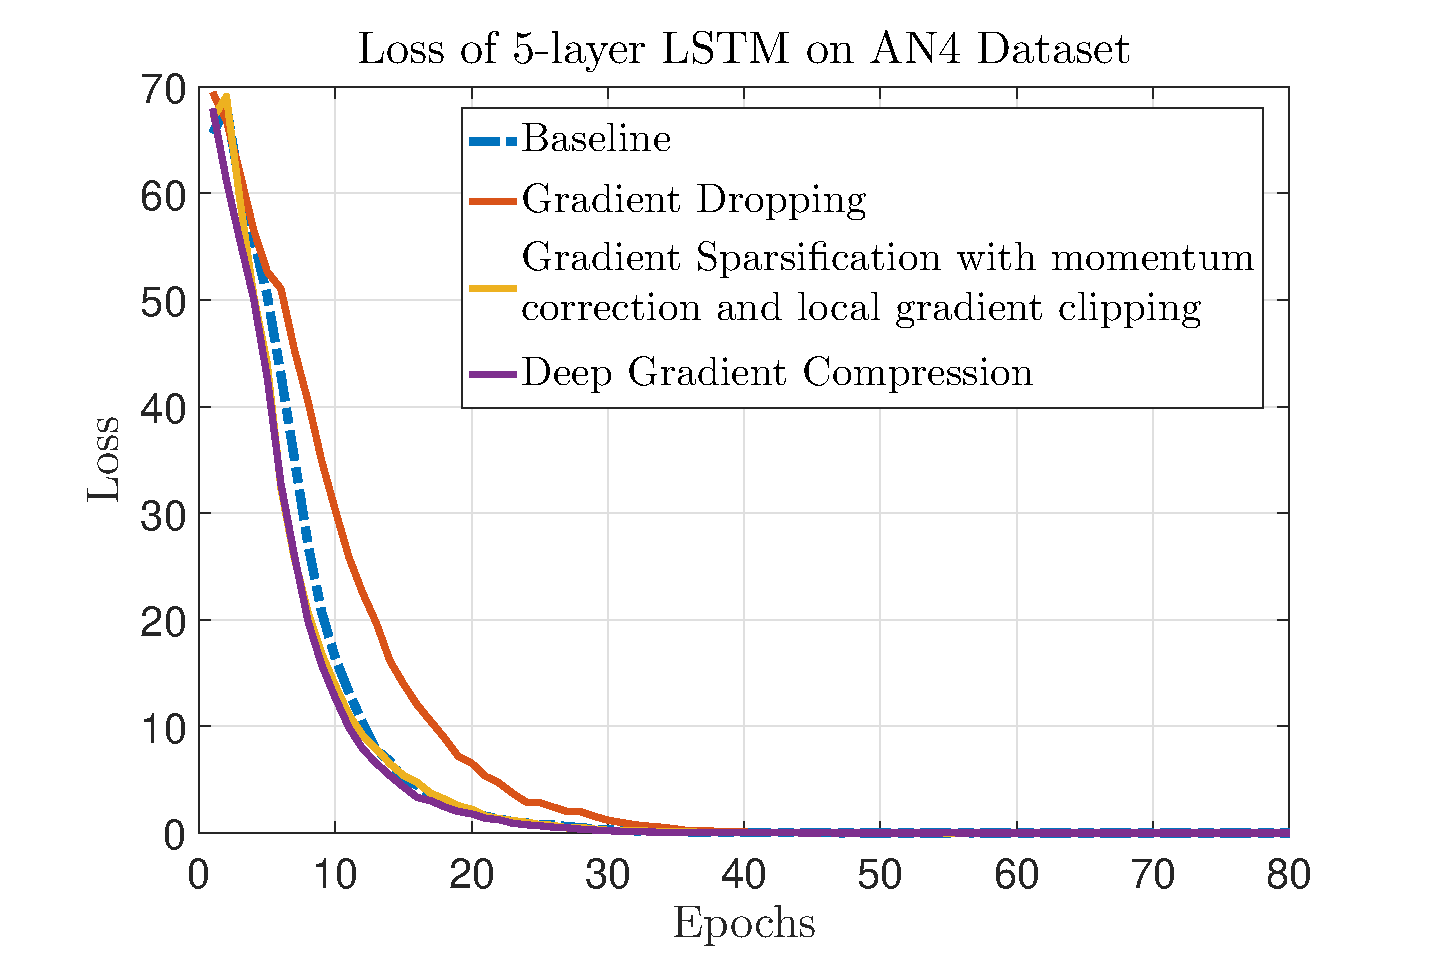
\includegraphics[width=0.49\textwidth]{figures/an_loss.eps}
  \caption*{图~A-8\hskip1em 5层LSTM在AN4数据集上的字差错率和训练损失(梯度稀疏度为99.9\%)}
  \label{fig:an}
\end{figure}

\begin{figure}[ht]
  \centering
  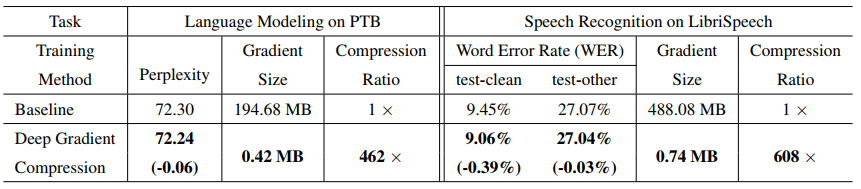
\includegraphics[width=\textwidth]{figures/table4.png}
  \caption*{图~A-9\hskip1em 使用4个节点训练语言模型和语音识别的训练结果}
  \label{fig:table4}
\end{figure}

我们首先测试图像分类任务中的深度梯度压缩。图A-5(a)和A-5(b)是Cifar10上有4个节点的ResNet--110的rop--1准确率和训练损失。梯度稀疏度为99.9\%(只有0.1\%非零元)。梯度丢弃的学习曲线由于梯度数据过时问题而比基线更差。使用动量校正(黄色),学习曲线收敛速度稍快,精度更接近基线。通过动量因子掩蔽和预训练技术(蓝色),消除了梯度过时问题,学习曲线接近基线。图A-4显示了详细的准确率。在使用深度梯度压缩时,ResNet--110的精度得以完全保持。

当使用大规模数据集时,图A-5(c)和A-5(d)显示了当梯度稀疏度为99.9\%时ResNet--50的学习曲线,其精确度完全符合基线。我们观察到一个有趣的现象,稀疏梯度训练的top--1误差比相同训练损失的基线下降得更快。图A-6显示了AlexNet和ResNet--50在具有4个节点的ImageNet上的训练结果。我们在AlexNet上将梯度压缩比例与Terngrad 进行了比较。深度梯度压缩比Terngrad压缩好75倍,且不损失精度。对于ResNet--50,压缩比稍低(相比于AlexNet压缩597倍,ResNet—50只压缩了277倍),精度略有提高。

对于语言模型,图A-7显示了当梯度稀疏度为99.9\%时,用4个节点训练的语言模型的困惑度(perplexity)和训练损失。深度梯度压缩的训练损失与基线紧密匹配,验证集的困惑度也是如此。从图A-9中,深度梯度压缩将梯度压缩462倍,同时略微降低了困惑度。

对于语音识别,图A-8显示了梯度稀疏度为99.9\%时,AN4数据集上5层LSTM的单词错误率(WER)和训练损失曲线。学习曲线显示了从深度梯度压缩技术中获得的与图像网络相同的改进。图A-9显示了LibriSpeech测试数据集上的字差错率(WER)性能,其中\emph{test-clean}包含干净的语音而\emph{test-other}包含噪声的语音。使用深度梯度压缩训练的模型在干净和有噪声的语音上即使梯度大小被压缩608倍,也能获得更好的识别能力。

\section{系统分析与性能}
\begin{figure}[ht]
  \centering
  \begin{subfigure}{7cm}
    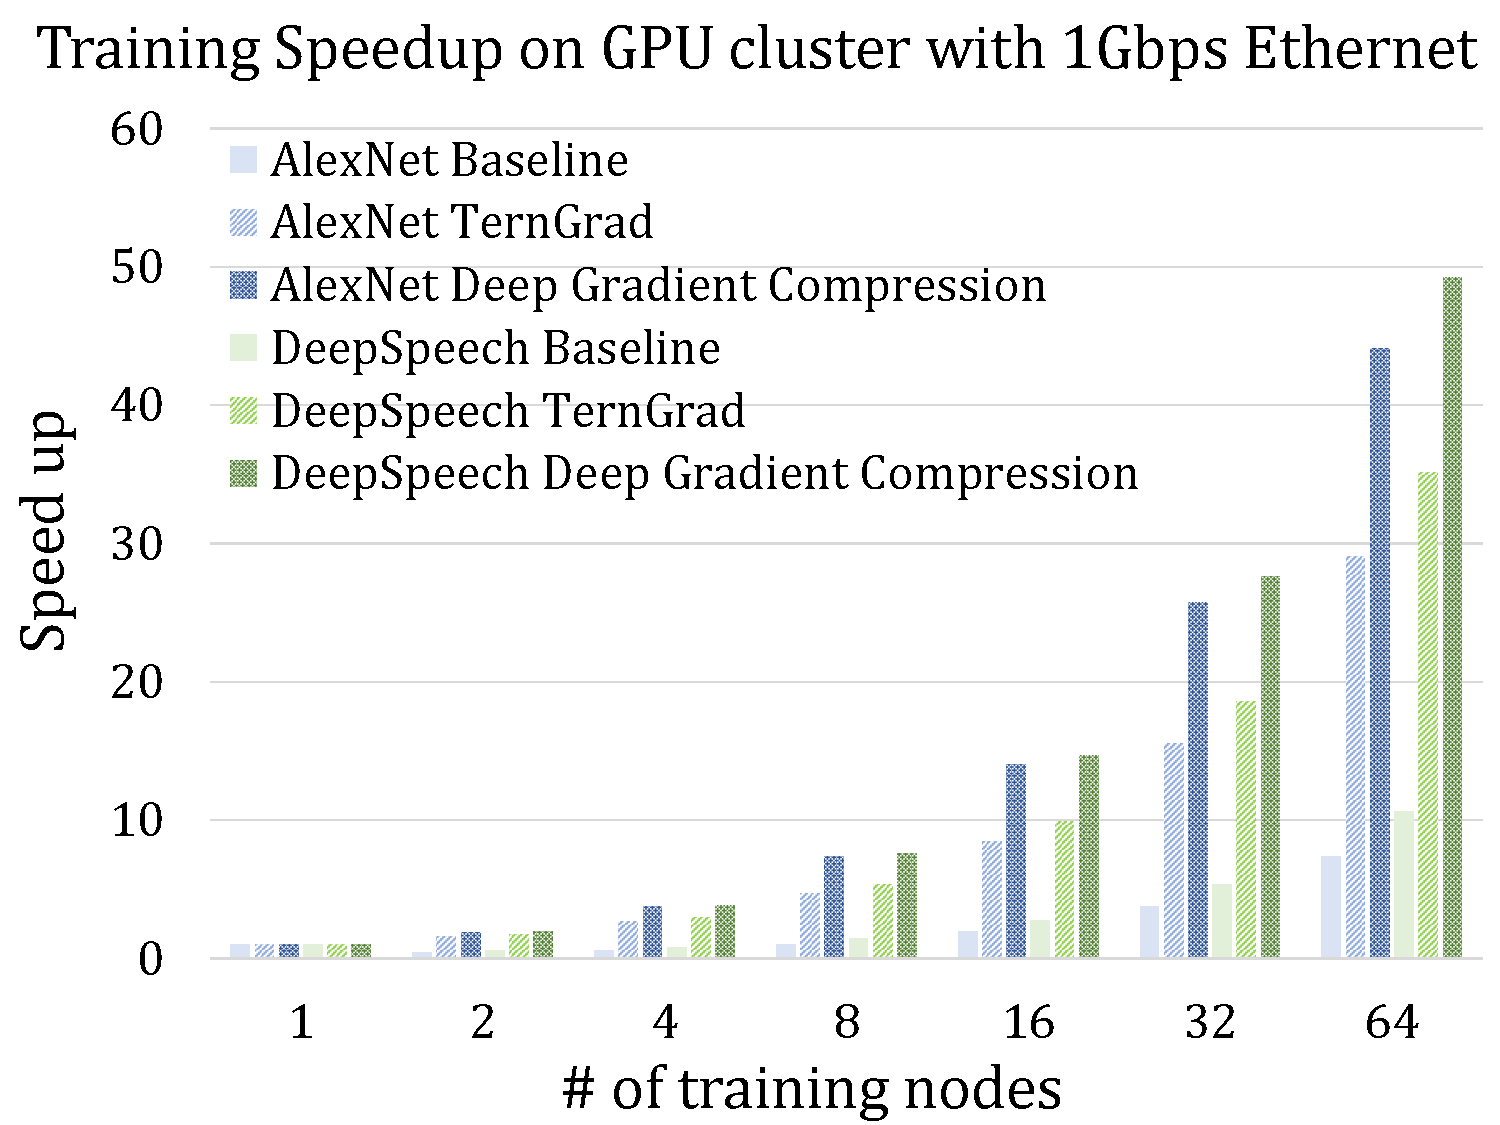
\includegraphics[width=\textwidth]{figures/1g.pdf}\label{fig:time_1}
  \end{subfigure}
  \begin{subfigure}{7cm}
    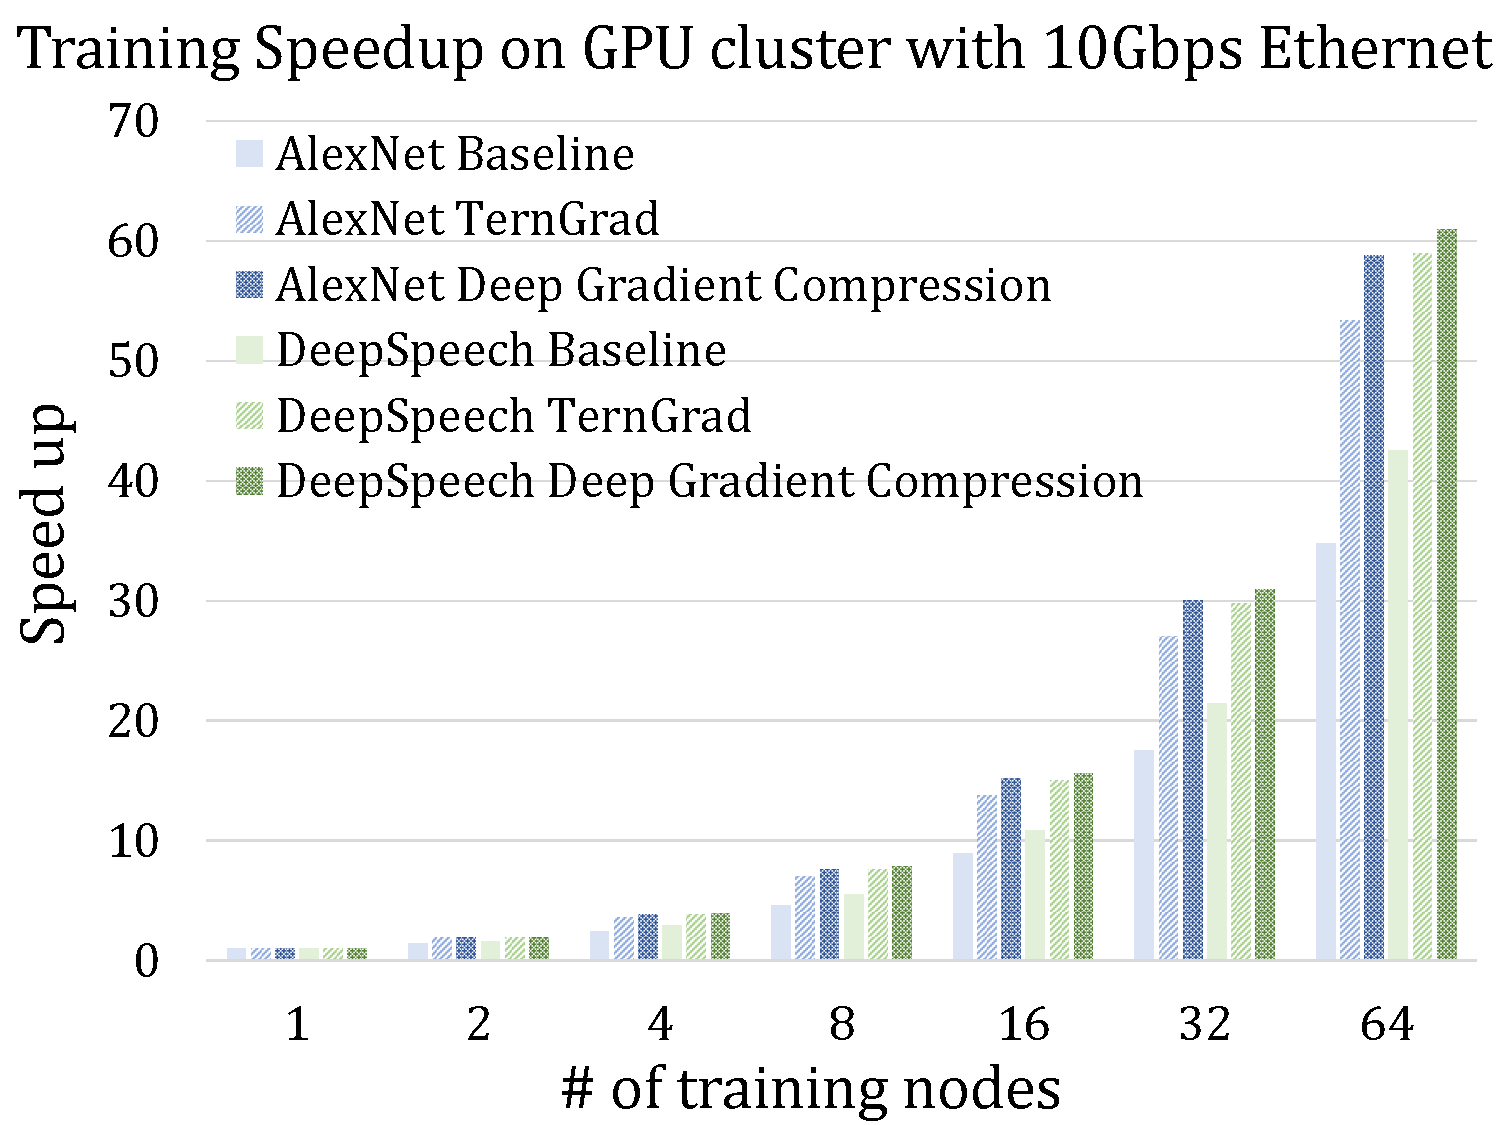
\includegraphics[width=\textwidth]{figures/10g.pdf}\label{fig:time_10}
  \end{subfigure}
  \caption*{图~A-10\hskip1em 深度梯度压缩提高了分布式训练的速度和可扩展性。每个训练节点有4个NVIDIA Titan XP图形处理器和一个PCI交换机。}
  \label{fig:time}
\end{figure}

实施DGC需要选择第k大梯度。给定99.9\%的目标稀疏率,我们需要在数百万个权重中选出最大的0.1\%。它的复杂度是$\Theta(n)$,其中n是梯度元素的数量。我们建议使用采样来减少第k大选择时间。我们只对0.1\%到1\%的梯度进行采样,并对样本进行第k大值选择,以估计整体的阈值。如果超过阈值的梯度数量远远超过预期,则根据已经选择的梯度计算精确的阈值。分层计算阈值显著减少了第k大选择时间。实际上,与网络通信时间相比,总的额外计算时间可以忽略不计,网络通信时间通常从几百毫秒到几秒,具体取决于网络带宽。

我们使用Wen等人提出的性能模型来执行可扩展性分析,将单个训练节点上的轻量级分析与分析通信建模相结合。使用Allreduce通信模型,在最坏的情况下,稀疏数据的密度在每个聚集步骤都加倍。然而,即使考虑到这种影响,深度梯度压缩仍然显著减少了网络通信时间,如图A-10所示。

图A-10显示了多节点训练相对于单节点训练的加速。传统的训练以1 Gbps以太网(图A-10(a))实现的加速比10 Gbps以太网(图A-10(b))要差得多。尽管如此,深度梯度压缩使使用1 Gbps以太网的训练能够与使用10 Gbps以太网的传统训练竞争。例如,在用64个节点训练AlexNet时,传统训练仅用10 Gbps以太网实现了约30倍的加速,而在DGC,仅用1 Gbps以太网就实现了40倍以上的加速。从图A-10(a)和图A-10(b)的比较来看,当模型的通信与计算比率较高且网络带宽较低时,深度梯度压缩的好处甚至更多。

\section{结论}
深度梯度压缩(DGC)可以将各种CNN和RNN的梯度压缩270--600倍。为了在不减慢收敛速度的情况下实现这种压缩,DGC采用动量校正、局部梯度修剪、动量因子掩蔽和预训练。我们进一步提出分层阈值选择来加速梯度稀疏化过程。深度梯度压缩减少了所需的通信带宽,并通过廉价的商用网络基础设施提高了分布式训练的可扩展性。

\section{附录}
\subsection{A 同步的分布式随机梯度下降}
在实践中,每个训练节点对具有相同网络模型的训练数据集采样的不同批次执行前向--反向传播。 将来自所有节点的梯度结合起来以优化其模型。 通过该同步步骤,在训练期间不同节点上的模型总是相同的。 聚合步骤可以以两种方式实现。 一种方法是使用参数服务器作为中介,其在多个服务器之间存储参数。 当服务器等待来自所有节点的梯度时,节点将梯度发送到服务器。 发送所有梯度后,服务器会更新参数,然后所有节点都会从服务器中提取最新参数。 另一种方法是对所有节点之间的梯度执行Allreduce操作,并独立更新每个节点上的参数,如算法2和图A-11所示。在本文中,我们默认采用后一种方法。

\begin{figure}[H]
  \begin{minipage}[H]{.43\linewidth}
    \begin{figure}[H]
      \begin{subfigure}{6cm}
        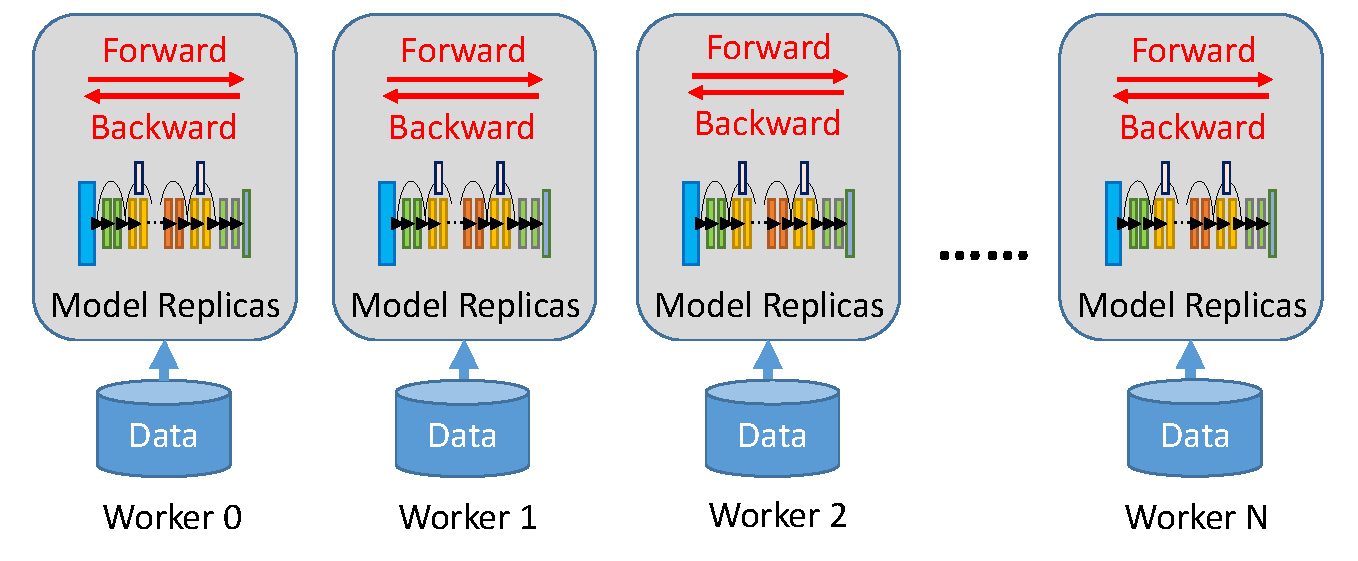
\includegraphics[width=\textwidth]{figures/dsgd1.pdf}\\[-2ex]
        \caption{每个节点独立计算梯度}
      \end{subfigure}
      \begin{subfigure}{6cm}
        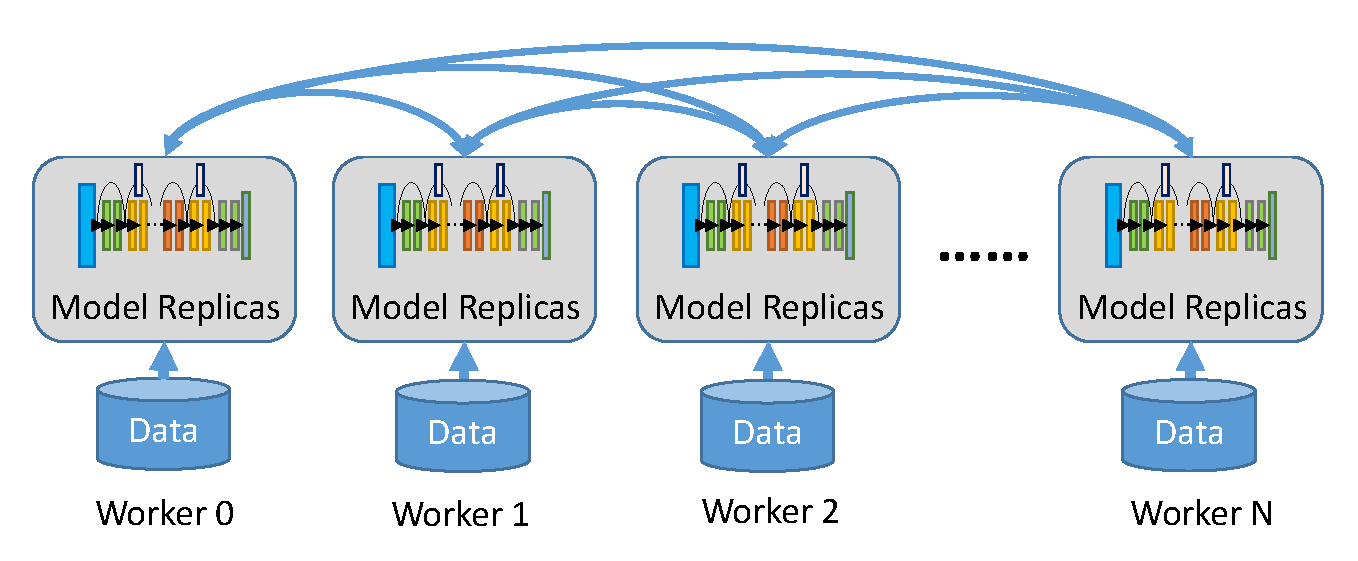
\includegraphics[width=\textwidth]{figures/dsgd2.pdf}
        \caption{用于汇集梯度的Allreduce操作}
      \end{subfigure}
      \caption*{图~A-11\hskip1em 分布式同步SGD}
      \label{fig:dsgd}
    \end{figure}
  \end{minipage}
  \begin{minipage}[H]{.55\linewidth}
    \begin{algorithm}[H]
      \caption*{\textbf{Algorithm~A-2}\hskip1em $k$个节点上的分布式同步SGD}
      \label{alg:SGD}
      \begin{algorithmic}[1]
        \Require Dataset $\chi$
        \Require minibatch size $b$ per node
        \Require the number of nodes $N$
        \Require Optimization Function $SGD$
        \Require Init parameters $w = \{w[0], \cdots, w[M]\}$
        \For{$t=0,1,\cdots$}
        \State $G_{t}^{k} \gets 0$
        \For{$i=1,\cdots,B$}
        \State Sample data $x$ from $\chi$
        \State $G_{t}^{k} \gets G_{t}^{k} + \frac{1}{Nb} \triangledown f \left(x;w_{t} \right) $
        \EndFor
        \State \emph{All-reduce} $G_{t}^{k}$ : $G_{t} \gets \sum_{k=1}^{N} G_{t}^{k}$
        \State $w_{t+1} \gets \emph{SGD} \left(w_{t}, G_{t} \right)$
        \EndFor
      \end{algorithmic}
    \end{algorithm}
  \end{minipage}
\end{figure}

\subsection{B 使用Nesterov动量矫正的梯度稀疏化}
Nesterov动量SGD的传统更新规则如下,

\begin{equation}
	\label{eq:nsgd}
	u_{t+1} = mu_{t}+ \sum_{k=1}^{N}\left( \triangledown_{k,t}\right),\quad  w_{t+1} = w_{t} - \eta \left(m\cdot u_{t+1} + \triangledown_{t}\right)
\end{equation}

其中$m$是动量,$N$是训练节点的数量,并且$\triangledown_{k,t} =  \frac{1}{Nb} \sum_{x \in \mathcal{B}_{k, t}} \triangledown f(x, w_{t})$。在动量校正之前,稀疏的更新规则如下,

\begin{equation}
	\label{eq:nonc}
	v_{k,t+1} = v_{k,t} + \triangledown_{k,t},\quad u_{t+1} = mu_{t} + \sum_{k=1}^{N} sparse\left( v_{k,t+1}\right) ,\quad  w_{t+1} = w_{t} - \eta u_{t+1}
\end{equation}

在动量校正与方程式A-7共享相同的方法后,它变为,

\begin{equation}
	\label{eq:nc}
	u_{k,t+1} = mu_{k,t}+ \triangledown_{k,t},\quad  v_{k,t+1} = v_{k,t} + \left(m\cdot u_{k,t+1} + \triangledown_{k,t}\right),\quad  w_{t+1} = w_{t} - \eta \sum_{k=1}^{N} sparse\left( v_{k,t+1}\right) 
\end{equation}

\subsection{C 局部梯度裁剪}
当使用梯度裁剪训练递归神经网络时,我们在将算法1中的当前梯度$G^k_t$添加到积累梯度$G^k_{t-1}$之前,要先在本地执行梯度裁剪。将梯度的L2范数$||G||_2$的起始阈值设为$thr_G$,并将局部梯度L2范数$||G^k||_2$的阈值设为$thr_{G^k}$。

假设所有$N$个节点的梯度都以$\sigma^2$为方差独立同分布,则所有节点的梯度之和的方差为$N\sigma^2$,因此,

\begin{equation}
  E\left[ ||G^k||_2 \right]\approx \sigma, \quad E\left[ ||G||_2 \right]\approx N^{1/2} \sigma
\end{equation}

因此,我们将阈值乘以$N^{-1/2}$,即当前节点的全局阈值的分数,

\begin{equation}
  thr_{G^k} = N^{-1/2}\cdot thr_{G}
\end{equation}

\subsection{D 深度梯度压缩算法}
\begin{minipage}[t]{.50\textwidth}
  \begin{algorithm}[H] \small
    \caption*{{\textbf{Algorithm~A-3}\hskip1em \small $k$个节点上使用深度梯度压缩的N朴素动量SGD}}
    \label{alg:smsgd}
    \begin{algorithmic}[1]
      \Require dataset $\chi$
      \Require minibatch size $b$ per node
      \Require momentum $m$
      \Require the number of nodes $N$
      \Require optimization function \emph{SGD}
      \Require initial parameters $w = \{w[0], \cdots, w[M]\}$
      \State $U^{k} \gets 0$, $V^{k} \gets 0$
      \For{$t=0,1,\cdots$}
      \State $G_{t}^{k} \gets 0$
      \For{$i=1,\cdots,b$}
      \State Sample data $x$ from $\chi$
      \State $G_{t}^{k} \gets G_{t}^{k} + \frac{1}{Nb} \triangledown f \left(x;\theta_{t} \right) $
      \EndFor
                \If {Gradient Clipping}
                \State $G_{t}^{k} \gets LocalGradientClipping(G_{t}^{k})$
                \EndIf
      \State $U_{t}^{k} \gets m \cdot U_{t-1}^{k} + G_{t}^{k}$
      \State $V_{t}^{k} \gets V_{t-1}^{k} + U_{t}^{k}$
      \For{$j=0, \cdots, M$}
      \State $thr \gets s\%$ of $\left|V_{t}^{k}[j]\right|$
      \State $ Mask \gets \left|V_{t}^{k}[j]\right| > thr$
      \State $\widetilde{G}_{t}^{k}[j] \gets V_{t}^{k}[j] \odot Mask$
      \State $V_{t}^{k}[j] \gets V_{t}^{k}[j] \odot \neg Mask$
                \State $U_{t}^{k}[j] \gets U_{t}^{k}[j] \odot \neg Mask$
      \EndFor
      \State \emph{All-reduce}: $G_{t} \gets \sum_{k=1}^{N} encode(\widetilde{G}_{t}^{k})$
      \State $\theta_{t+1} \gets \emph{SGD} \left(\theta_{t}, G_{t} \right)$
      \EndFor
    \end{algorithmic}
  \end{algorithm}
\end{minipage}
\begin{minipage}[t]{.50\textwidth}
  \begin{algorithm}[H] \small
    \caption*{{\textbf{Algorithm~A-4}\hskip1em \small $k$个节点上使用深度梯度压缩的Nesterov动量SGD}}
    \label{alg:snsgd}
    \begin{algorithmic}[1]
      \Require dataset $\chi$
      \Require minibatch size $b$ per node
      \Require momentum $m$
      \Require the number of nodes $N$
      \Require optimization function \emph{SGD}
      \Require initial parameters $w = \{w[0], \cdots, w[M]\}$
      \State $U^{k} \gets 0$, $V^{k} \gets 0$
      \For{$t=0,1,\cdots$}
      \State $G^{k} \gets 0$
      \For{$i=1,\cdots,b$}
      \State Sample data $x$ from $\chi$
      \State $G_{t}^{k} \gets G_{t}^{k} + \frac{1}{Nb} \triangledown f \left(x;\theta_{t} \right) $
      \EndFor
                \If {Gradient Clipping}
                \State $G_{t}^{k} \gets LocalGradientClipping(G_{t}^{k})$
                \EndIf
      \State $U_{t}^{k} \gets m \cdot \left(U_{t-1}^{k} + G_{t}^{k} \right)$
      \State $V_{t}^{k} \gets V_{t-1}^{k} + U_{t}^{k} + G_{t}^{k}$
      \For{$j=0, \cdots, M$}
      \State $thr \gets s\%$ of $\left|V_{t}^{k}[j]\right|$
      \State $ Mask \gets \left|V_{t}^{k}[j]\right| > thr$
      \State $\widetilde{G}_{t}^{k}[j] \gets V_{t}^{k}[j] \odot Mask$
      \State $V_{t}^{k}[j] \gets V_{t}^{k}[j] \odot \neg Mask$
                \State $U_{t}^{k}[j] \gets U_{t}^{k}[j] \odot \neg Mask$
      \EndFor
      \State \emph{All-reduce}: $G_{t} \gets \sum_{k=1}^{N} encode(\widetilde{G}_{t}^{k})$
      \State $\theta_{t+1} \gets \emph{SGD} \left(\theta_{t}, G_{t} \right)$
      \EndFor
    \end{algorithmic}
  \end{algorithm}
\end{minipage}


\centerline{书面翻译对应的外文资料的原文索引}

\centerline{\heiti 书面翻译对应的外文资料的原文索引}

Lin Y, Han S, Mao H, et al. Deep gradient compression: Reducing the communication bandwidth for distributed training[J]. arXiv preprint arXiv:1712.01887, 2017.